\chapter{Vivado results}
After completing the verification phase, the circuit design was synthesized and implemented using the Vivado Tool, specifically targeting the Zybo Zynq-7010 development board.

\section{Vivado Design flow}
For the implementation of the CORDIC algorithm in vectoring mode for Cartesian-to-Polar conversion, the Vivado design flow was employed using Xilinx/AMD Vivado software. This process involved RTL Elaboration, Synthesis, and Implementation on the target FPGA, along with the application of design constraints and the extraction of power and timing reports. To ensure accurate and reliable timing analysis, all combinational logic paths were structured to follow a Register-Logic-Register configuration.

\section{RTL}
Vivado produced a logic network made of:

% todo cambiare numeri
\begin{enumerate}
    \item 155 cells (e.g. multiplexers, DFFs, adders)
    \item 68 I/O ports ($16_{x} + 16_{y} + 16_{\rho} + 16_{\theta} + 1_{clk} + 1_{rst} + 1_{start} + 1_{valid}$)
    \item 982 nets (for connecting all the components)
\end{enumerate}

The RTL Analysis generated the following Elaborated Design consistent with the expected structure of the system:
% fare nuovo pdf schematic
\begin{figure}[H]
    \centering
    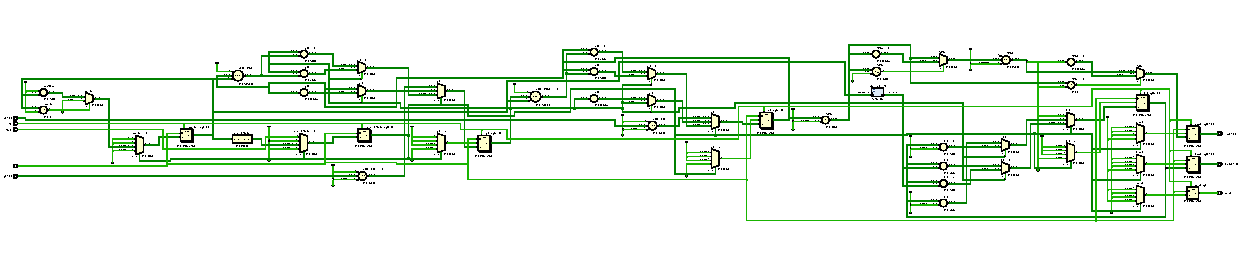
\includegraphics[width=\textwidth]{./images/Synthesis/schematic.pdf}
    \caption{Elaborated RTL design.}
    \label{fig:schematic}
\end{figure}

\section{Synthesis}
\subsection{Critical Paths}
% to do cambiare schema
\begin{figure}[H]
    \centering
    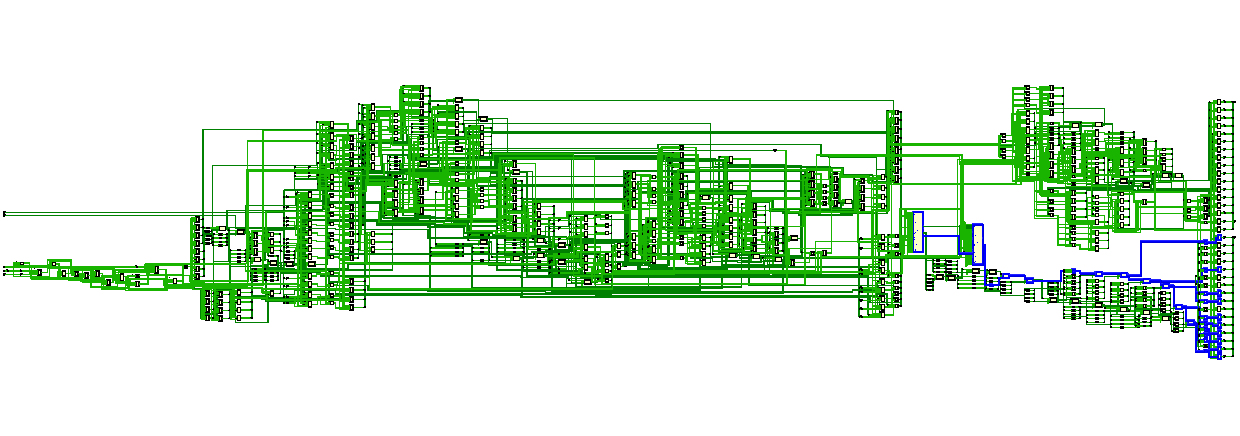
\includegraphics[width=\textwidth]{./images/Vivado/setup_synthesis.pdf}
    \caption{Figure showing the elaborated RTL design with the main critical paths for set-up-time-violation found in synthesis step highlighted in blue.}
    \label{fig:setup_synthesis}
\end{figure}

% to do aggiornare dati tabella
\begin{table}[H]
    \centering
    \small
    \captionsetup{skip=10pt} 
    \begin{tabular}{lrrrrrrr}
        \hline
        Name &  Slack &  Levels &  Routes & From      & To                 & Total Delay    \\
        \hline
        Path 1 &   9.30 &      12 &       6 & ARG2/CLK  & x\_out\_reg[15]/D  &        10.55  \\
        Path 2 &   9.33 &      11 &       6 & ARG2/CLK  & x\_out\_reg[12]/D  &        10.52  \\
        Path 3 &   9.45 &      10 &       6 & ARG2/CLK  &  x\_out\_reg[8]/D  &        10.40  \\
        Path 4 &   9.51 &      12 &       6 & ARG2/CLK  & x\_out\_reg[14]/D  &        10.33  \\
        Path 5 &   9.56 &       9 &       6 & ARG2/CLK  &  x\_out\_reg[4]/D  &        10.28  \\
        Path 6 &   9.57 &      11 &       6 & ARG2/CLK  & x\_out\_reg[11]/D  &        10.28  \\
        Path 7 &   9.62 &      12 &       6 & ARG2/CLK  & x\_out\_reg[13]/D  &        10.23  \\
        Path 8 &   9.62 &      11 &       6 & ARG2/CLK  & x\_out\_reg[10]/D  &        10.23  \\
        Path 9 &   9.67 &       8 &       6 & ARG2/CLK  &  x\_out\_reg[0]/D  &        10.18  \\
        Path 10 &   9.69 &      10 &       6 & ARG2/CLK  &  x\_out\_reg[7]/D  &       10.16  \\
        \hline
    \end{tabular}
    \caption{Table showing data of the main critical paths found in synthesis step}
    \label{tab:setup_synthesis}
\end{table}
    
% to do cambiare schema
\begin{figure}[H]
    \centering
    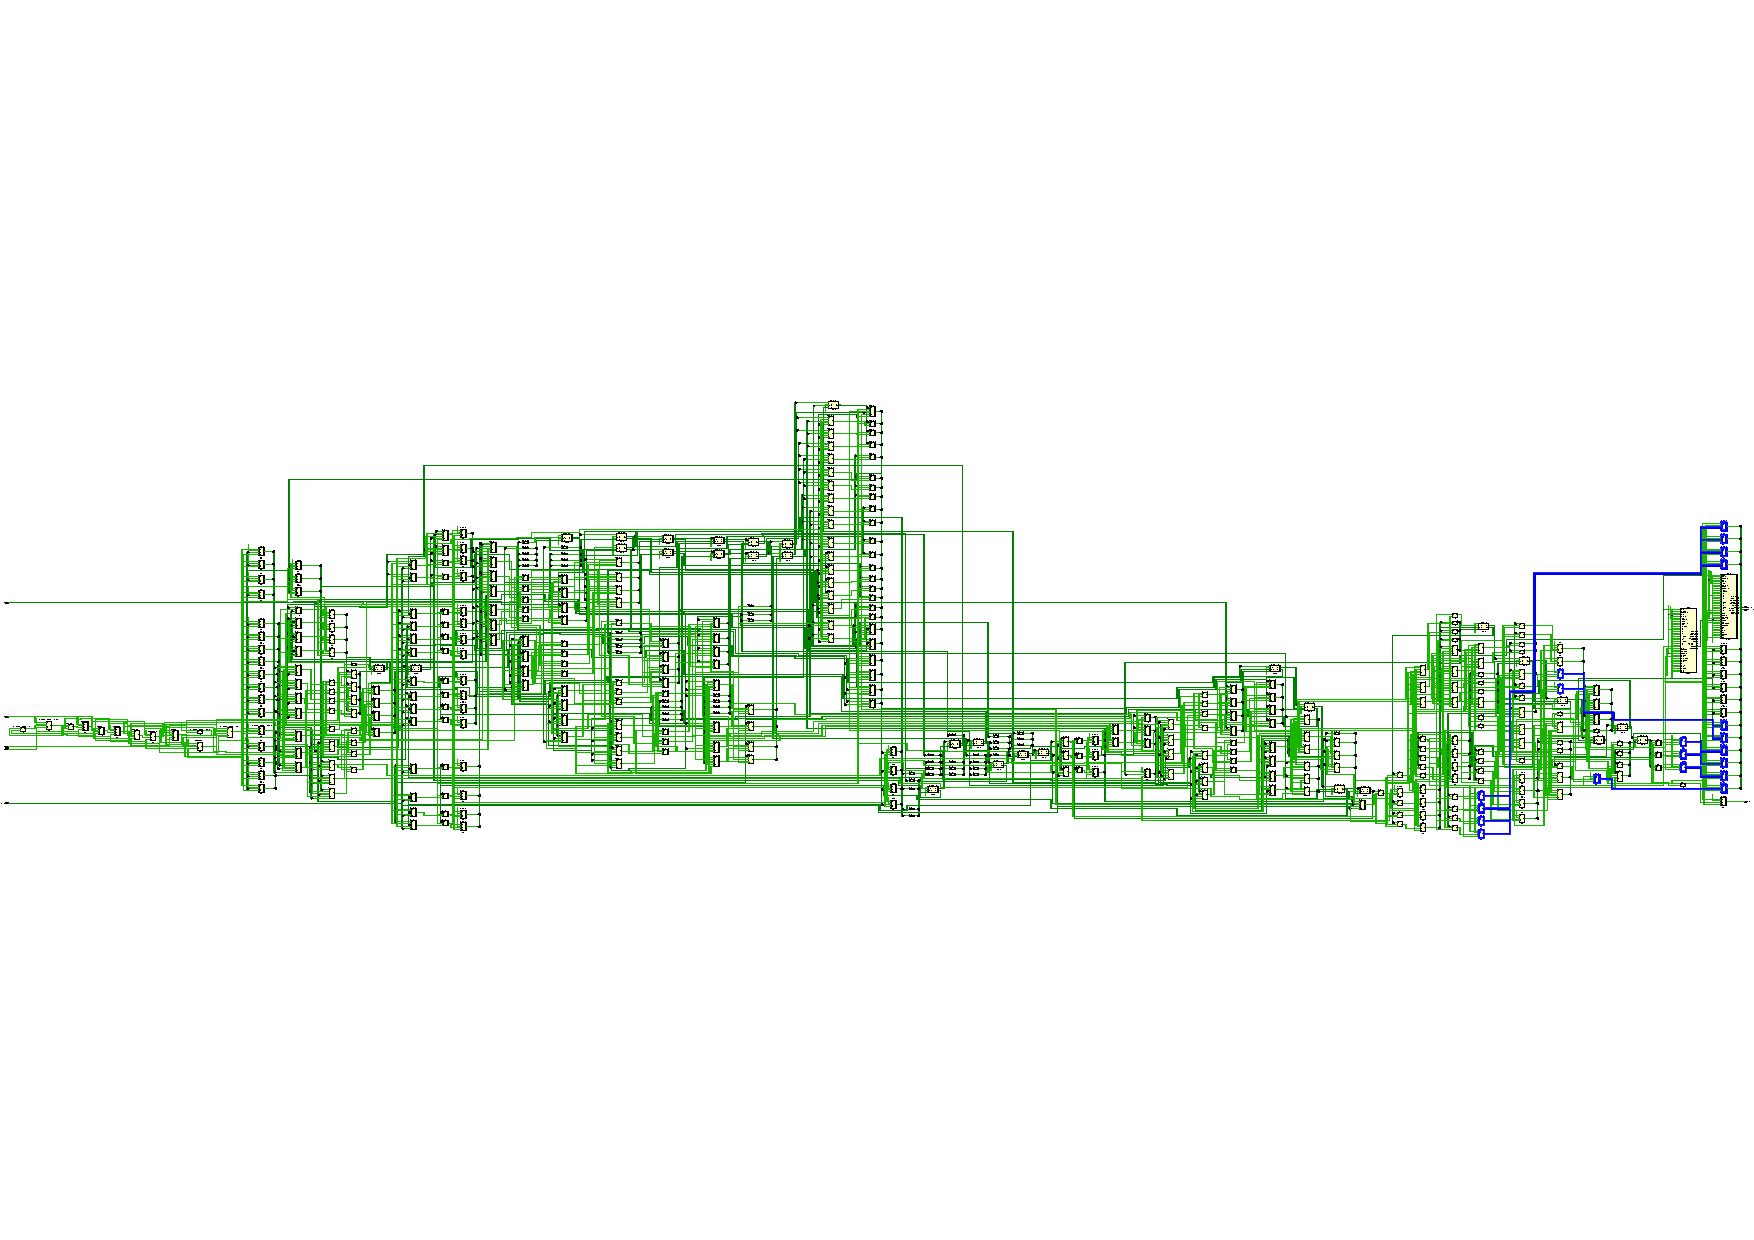
\includegraphics[width=\textwidth]{./images/Vivado/hold_synthesis.pdf}
    \caption{Figure showing the elaborated RTL design with the main critical paths for hold-time-violation found in synthesis step highlighted in blue.}
    \label{fig:hold_synthesis}
\end{figure}  

% to do aggiornare dati tabella
\begin{table}[H]
    \centering
    \small
    \captionsetup{skip=10pt} 
    \begin{tabular}{lrrrrrr}
        \hline
        Name    & Slack & Levels & Routes  & From           & To               & Total Delay \\
        \hline
        Path 11 & 0.16  & 0      & 1       & z\_t\_reg[23]/C & z\_out\_reg[15]/D & 0.29       \\
        Path 12 & 0.16  & 0      & 1       & z\_t\_reg[8]/C  & z\_out\_reg[0]/D  & 0.29       \\
        Path 13 & 0.16  & 0      & 1       & z\_t\_reg[18]/C & z\_out\_reg[10]/D & 0.29       \\
        Path 14 & 0.16  & 0      & 1       & z\_t\_reg[19]/C & z\_out\_reg[11]/D & 0.29       \\
        Path 15 & 0.16  & 0      & 1       & z\_t\_reg[20]/C & z\_out\_reg[12]/D & 0.29       \\
        Path 16 & 0.16  & 0      & 1       & z\_t\_reg[21]/C & z\_out\_reg[13]/D & 0.29       \\
        Path 17 & 0.16  & 0      & 1       & z\_t\_reg[22]/C & z\_out\_reg[14]/D & 0.29       \\
        Path 18 & 0.16  & 0      & 1       & z\_t\_reg[9]/C  & z\_out\_reg[1]/D  & 0.29       \\
        Path 19 & 0.16  & 0      & 1       & z\_t\_reg[10]/C & z\_out\_reg[2]/D  & 0.29       \\
        Path 20 & 0.16  & 0      & 1       & z\_t\_reg[11]/C & z\_out\_reg[3]/D  & 0.29       \\
        \hline
    \end{tabular}
    \caption{Table showing the characteristics regarding critical paths for hold-time-violation found in synthesis step.}
    \label{tab:hold_synthesis}
\end{table}


\section{Implementation}
% todo aggiornare dati tabella
\begin{table}[H]
    \centering
    \small
    \captionsetup{skip=10pt} 
    \begin{tabular}{lrrrrrr}
        \hline
        Name    & Slack & Levels & Routes & From      & To                 & Total Delay \\
        \hline
        Path 1  & 8.90  & 10     & 3      & ARG2/CLK  & x\_out\_reg[9]/D   & 10.99       \\
        Path 2  & 8.93  & 10     & 3      & ARG2/CLK  & x\_out\_reg[12]/D  & 10.96       \\
        Path 3  & 8.99  & 11     & 3      & ARG2/CLK  & x\_out\_reg[13]/D  & 10.86       \\
        Path 4  & 9.08  & 11     & 3      & ARG2/CLK  & x\_out\_reg[15]/D  & 10.82       \\
        Path 5  & 9.10  & 9      & 3      & ARG2/CLK  & x\_out\_reg[8]/D   & 10.84       \\
        Path 6  & 9.10  & 9      & 3      & ARG2/CLK  & x\_out\_reg[6]/D   & 10.84       \\
        Path 7  & 9.14  & 10     & 3      & ARG2/CLK  & x\_out\_reg[10]/D  & 10.71       \\
        Path 8  & 9.15  & 9      & 3      & ARG2/CLK  & x\_out\_reg[7]/D   & 10.74       \\
        Path 9  & 9.18  & 11     & 3      & ARG2/CLK  & x\_out\_reg[14]/D  & 10.72       \\
        Path 10 & 9.22  & 10     & 3      & ARG2/CLK  & x\_out\_reg[11]/D  & 10.63       \\
        \hline
    \end{tabular}
    \caption{Table showing the main critical paths for the setup-time-violation during the implementation step.}
    \label{tab:setup_implementation}
\end{table}


\begin{table}[H]
    \centering
    \small
    \captionsetup{skip=10pt} 
    \begin{tabular}{lrrrrrr}
        \hline
        Name    & Slack & Levels & Routes  & From                              & To                    & Total Delay \\
        \hline
        Path 11 & 0.17  & 1      & 1       & counter\_reg[0]/C                & counter\_reg[2]/D     & 0.31       \\
        Path 12 & 0.17  & 1      & 1       & counter\_reg[0]/C                & counter\_reg[1]/D     & 0.31       \\
        Path 13 & 0.18  & 1      & 1       & counter\_reg[0]/C                & counter\_reg[3]/D     & 0.31       \\
        Path 14 & 0.22  & 0      & 1       & z\_t\_reg[19]/C                  & z\_out\_reg[11]/D     & 0.25       \\
        Path 15 & 0.22  & 0      & 1       & z\_t\_reg[23]/C                  & z\_out\_reg[15]/D     & 0.27       \\
        Path 16 & 0.23  & 0      & 1       & z\_t\_reg[8]/C                   & z\_out\_reg[0]/D      & 0.26       \\
        Path 17 & 0.25  & 0      & 1       & z\_t\_reg[12]/C                  & z\_out\_reg[4]/D      & 0.35       \\
        Path 18 & 0.25  & 0      & 1       & z\_t\_reg[22]/C                  & z\_out\_reg[14]/D     & 0.33       \\
        Path 19 & 0.26  & 1      & 1       & FSM\_reg[0]/C                    & FSM\_reg[0]/D         & 0.35 \\
        Path 20 & 0.27  & 0      & 1       & z\_t\_reg[18]/C                  & z\_out\_reg[10]/D     & 0.37       \\
        \hline
    \end{tabular}
    \caption{Table showing the main critical paths for hold-time-violation found in the implementation step.}
    \label{tab:hold_implementation}
\end{table}

\subsection{Utilization Report}
\begin{table}[H]
    \centering
    \small
    \captionsetup{skip=10pt} 
    \begin{tabular}{lrr}
        \hline
        Resource               & Utilization (\%) & Description \\
        \hline
        Slice LUTs             & 2.05\%           & Look-Up Tables used as logic \\
        Slice Registers        & 0.32\%           & Registers used in the design \\
        Slice                  & 2.30\%           & Total slices utilized \\
        LUT as Logic           & 2.05\%           & LUTs specifically used as logic \\
        DSPs                   & 2.50\%           & Digital Signal Processing blocks \\
        Bonded IOB             & 68.00\%          & Bonded Input/Output Blocks \\
        BUFGCTRL               & 3.13\%           & Global Clock Buffers \\
        \hline
    \end{tabular}
    \caption{Resource utilization for the CORDIC design (only non-zero values shown)}
    \label{tab:cordic_resource_utilization}
\end{table}


\subsection{Power Report}
\begin{figure}[H]
    \centering
    \captionsetup{skip=10pt} 
    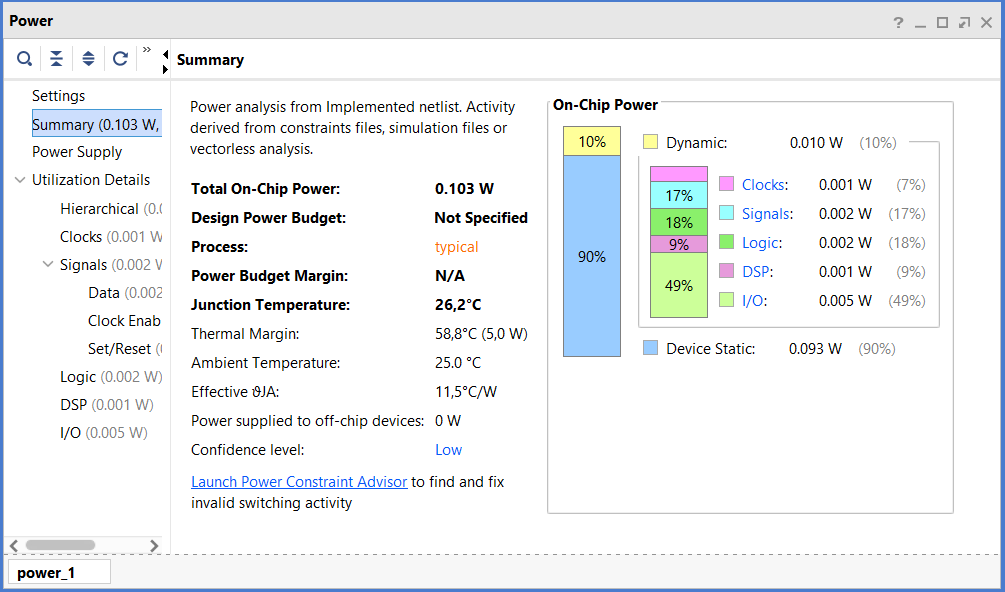
\includegraphics[width=\textwidth]{./images/Vivado/power_report.png}
    \caption{Vivado Power Report after implementation.}
    \label{fig:power_report}
\end{figure}




